%%%%%%%%%%%%%%%%%%%%%%%%%%%%%%%%%%%%%%%%%
% Medium Length Professional CV
% LaTeX Template
% Version 2.0 (8/5/13)
%
% This template has been downloaded from:
% http://www.LaTeXTemplates.com
%
% Original author:
% Trey Hunner (http://www.treyhunner.com/)
%
% Important note:
% This template requires the resume.cls file to be in the same directory as the
% .tex file. The resume.cls file provides the resume style used for structuring the
% document.
%
%%%%%%%%%%%%%%%%%%%%%%%%%%%%%%%%%%%%%%%%%

%----------------------------------------------------------------------------------------
%	PACKAGES AND OTHER DOCUMENT CONFIGURATIONS
%----------------------------------------------------------------------------------------

\documentclass{resume} % Use the custom resume.cls style

\usepackage{bibentry}
\usepackage{scalerel}

\usepackage[left=0.75in,top=0.6in,right=0.75in,bottom=0.6in]{geometry} % Document margins
\newcommand{\tab}[1]{\hspace{.2667\textwidth}\rlap{#1}}
\newcommand{\itab}[1]{\hspace{0em}\rlap{#1}}
\name{Sean Gillen} % Your name
%\address{6510 El Colegio Road, Apt 1212A,  Goleta CA,  93106 } % Your address
%\address{123 Pleasant Lane \\ City, State 12345} % Your secondary addess (optional)
\address{sgillen@ucsb.edu  $|$  github.com/sgillen  $|$ linkedin.com/in/sgillen} % Your phone number and email

\begin{document}

%----------------------------------------------------------------------------------------
%	EDUCATION SECTION
%----------------------------------------------------------------------------------------

\begin{rSection}{Education}

{\bf University of California Santa Barbara} \hfill {September 2017 - March 2022} 
\\{  MS/PhD Electrical And Computer Engineering}
%\\ {Thesis: Improving Reinforcement Learning for Robotics with Control and Dynamical Systems Theory}

% \hfill {GPA: 4.0}


{\bf University of Maryland College Park} \hfill {September 2013 - May 2017} 
\\{ BS Electrical Engineering} \hfill% { GPA: 3.5}

\end{rSection}


%----------------------------------------------------------------------------------------
%	TECHNICAL SKILLS
%----------------------------------------------------------------------------------------

\begin{rSection}{Technical Skills}

\begin{tabular}{ @{} >{\bfseries}l @{\hspace{6ex}} l }
  Languages &  Python, C++, C, MATLAB, Bash, Mathematica, Julia, Elisp, \LaTeX \\
%           &  Make, Cmake, ROS, OpenCV, Pytorch, Git, Lin
Libraries etc. &  ROS, Pytorch, Gazebo, OpenCV, Linux, Make, Cmake \\
Electrical & Embedded system prototyping/debugging. (Oscilliscopes, DLAs, etc.) \\
Mechanical & Prototyping (manual and CNC machining, 3D printing, soldering/crimping, etc.)
\end{tabular}

\end{rSection}


%----------------------------------------------------------------------------------------
%	WORK EXPERIENCE SECTION
%----------------------------------------------------------------------------------------


\begin{rSection}{Work History}

  
\begin{rSubsection}{Veoneer}{June 2019 - Present}{Robotics Consultant}{}
\item Delivered a \textbf{C++} device driver and \textbf{ROS} node for a new automotive camera system designed for Daimler.
\item Implemented camera authentication and security on a low power embedded system (\textbf{C}).
\item Developed an embedded system to allow technicians to automatically adjust focus on camera systems using stepper motors.
\end{rSubsection}

\begin{rSubsection}{University of California Santa Barbara}{September 2017 - March 2022}{Graduate Student Researcher}{}
\item Thesis: Improving Reinforcement Learning for Robotics with Control and Dynamical Systems Theory.
\item Developed novel control algorithms fusing reinforcement learning and control theory for low level robotic control (\textbf{Python, C++, Matlab}).
\end{rSubsection}

  
\begin{rSubsection}{Northrop Grumman}{June 2016 - September 2016}{Electrical Engineer}{}
\item System level integration for prototype sensor payloads in an unmanned underwater vehicle (UUV).
%\item Conducted successful in-field demo of the system to Navy officers.
\end{rSubsection}

\begin{rSubsection}{Naval Air Systems Command (NAVAIR)}{June 2015 - September 2015}{Electrical Engineering Intern}{}
\item Developed a prototype vision system capable of imaging in extremely turbid underwater environments.
\item Designed and constructed an underwater vessel to house and control the imaging system.
\end{rSubsection}

\begin{rSubsection}{University Of Maryland}{September 2015 - June 2016}{Undergraduate Student Researcher}{}
\item Implemented computer simulation of nematic liquid crystals using \textbf{Matlab} and \textbf{Mathematica}.
\item Gave a talk at the American Physics Society March Meeting. 
\end{rSubsection}

\begin{rSubsection}{Horn Point Laboratory}{June 2014 - June 2015}{Software Engineer}{}
\item Wrote software (\textbf{C++}) for a Remus 600 UUV to provide altitude control, user-defined acoustic modem messages, augmented data simulation, and adaptive mission planning to the vehicle.
\end{rSubsection}

\end{rSection}


\pagebreak

\begin{rSection}{Personal Projects}
  

\begin{rSubsection}{Seagul: Utility Library for Reinforcement Learning}{}{}{}
\item Wrote a \textbf{Python} package implementing state-of-the art reinforcement learning algorithms. Now used internally at the UCSB Robotics Lab for research in robotic control.
\end{rSubsection}

\begin{rSubsection}{Qubo: Underwater Octocopter}{}{}{}
\item Led a team of around 8 engineers to design and build an autonomous underwater octocoptor from scratch. The vehicle can autonomously navigate to targets using computer vision. Semifinalists at Robosub 2017.
\item Wrote majority of the vision (\textbf{OpenCV}), control (\textbf{C++}), autonomy (\textbf{Python}), and embedded (\textbf{Arduino}) software, using \textbf{ROS} as a middleware.
\end{rSubsection}


\begin{rSubsection}{Aq Bars: Tactile, Fist Bumping Robot Arm}{ }{}{}
\item Wrote software connecting a Novint Falcon controller to a low-cost robot arm, allowing users to control the arm and ``feel'' objects it interacts with.
%\item Wrote Arduino code for the arm to allow for interactive use.
%\item Successful Public Demo of the system to UCSB's Media Arts and Technology Department. 
\end{rSubsection}


\begin{rSubsection}{GAN Art}{}{}{} 
\item \vspace{-4mm} Trained a Generative Adversarial Network (GAN) to make fine art using \textbf{Pytorch}. \scalerel*{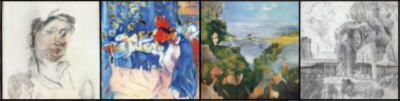
\includegraphics{sgillen_CV/more_art_smaller.png}}{\fbox{\rule[0em]{0ex}{2em}Work Table}}
\item Created an interactive notebook hosted on google collab, allowing anyone to explore the trained model, interpolate between images, and more!
\end{rSubsection}


\begin{rSubsection}{Compressed Air Engine}{ }{}{}
\item Manufactured a desktop compressed air engine, using manual and CNC Machine tools.
\end{rSubsection}

\end{rSection}


%----------------------------------------------------------------------------------------
%   Publications
%----------------------------------------------------------------------------------------

\begin{rSection}{Publications}
\bibliographystyle{unsrt}
\nobibliography{ref}

\item \bibentry{Gillen2022analytic} (Preprint, under review)
\item \bibentry{Gillen2021direct} (Preprint, under review)
\item \bibentry{ICRA2021}
\item \bibentry{CORL2020}
\item \bibentry{CDC2020}

\end{rSection}


%----------------------------------------------------------------------------------------
%   Teaching
%----------------------------------------------------------------------------------------

\begin{rSection}{Teaching}


Intermediate C programming  (Spring \& Fall 2016) \\ 
Introduction to Circuits (Fall 2017) \\ 
Digital Control (Winter 2017) \\ 
Introduction to Probability \& Statistics (Spring 2017) \\
Robotic Modeling \& Control (Fall 2018) \\
Operating Systems (Spring 2019) \\
Compilers (Fall 2020) \\
Algorithms \& Data Structures (Winter 2021, Spring 2021) 


\end{rSection}


% %----------------------------------------------------------------------------------------
% %   Honors and Awards
% %----------------------------------------------------------------------------------------

% %----------------------------------------------------------------------------------------
 % \begin{rSection}{Honors \& Awards} \itemsep -3pt
 % \item Bodharamik Engineering scholarship (2016)
 % \item Sikorsky Corporate Partners scholarship (2016)
 % \item Outstanding TA award (2017)
 % \end{rSection}

\end{document}
